\label{chap:eeg}
Für das Projekt wurde ein EMOTIV Epoc+ EEG Headset \footnote{\url{http://emotiv.com/epoc}} (Abb \ref{fig:epoc_eeg}) verwendet. Es besitzt 14 EEG Kanäle, sowie ein Gyroskop und sendet seine Daten via Bluetooth an den Rechner. Das Headset wird über den Kopf gestülpt und besitzen an den Sensorenenden einen Filz der mit Kochsalzlösung befeuchtet wird. 

\begin{figure}[h] 
  \begin{center}
    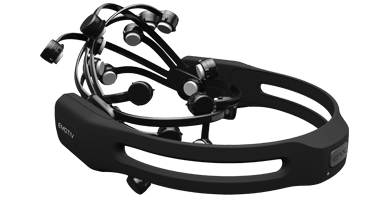
\includegraphics[width=0.75\columnwidth]{epoc_eeg}
    \caption[EMOTIV Epoc]{Das EMOTIV Epoc+ EEG Headset wird einfach über den Kopf gestülpt.\label{fig:epoc_eeg}}
  \end{center}
\end{figure}

Die Sensoren Anordnung ist an das internationale 10-20 System angelehnt (\ref{fig:epoc_sensors}). Die Rohdaten werden Abtastrate von 128 geliefert und enthalten neben dem Wert auch die Signalstärke (Qualität). Leider liefert die mitgelieferte SDK die Rohdaten nicht in Echtzeit, weshalb die Open-Source Lösung Emokit\footnote{\url{https://github.com/openyou/emokit}} eingebunden wurde.

\begin{figure}[h] 
  \begin{center}
    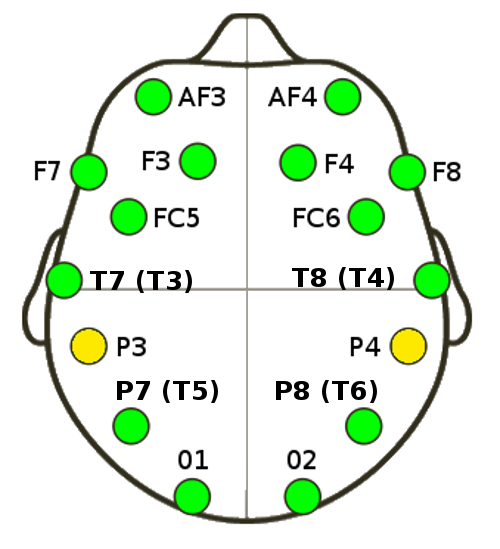
\includegraphics[width=0.75\columnwidth]{epoc_sensors}
    \caption[EEG Sensoren]{Die 14 Kanäle (Grün), sowie die beiden Qualitätssensoren (Gelb).\label{fig:epoc_sensors}}
  \end{center}
\end{figure}